\begin{frame}{Advanced Octave usage - oct-files}
\begin{columns}
\begin{column}{0.3\textwidth}
\begin{center}
\includegraphics[width=0.8\textwidth]{res/libreoffice/octave_c_cpp_fortran_2}
\end{center}
\end{column}
\begin{column}{0.65\textwidth}
\textbf{Problems to solve:}\\[0.8em]

\begin{itemize}
\itemsep1.5em
\item
Calling a C/C++ or Fortran function from some "easier" programming language.
\begin{itemize}
\item
Verify correctness (testing).

\item
Benchmarking.
\end{itemize}

\item
Wrapper class for C/C++-libraries, e.g., MPFR\footnote{\url{https://www.mpfr.org/}}.

\item
My native Octave code is too slow.
\begin{itemize}
\item
Translate time critical portions to compiled code, e.g., \\
unavoidable \textbf{nested loops}
\end{itemize}
\end{itemize}
\end{column}
\end{columns}
\end{frame}



\begin{frame}{Advanced Octave usage - standalone applications (1/2)}
\begin{columns}
\begin{column}{0.5\textwidth}
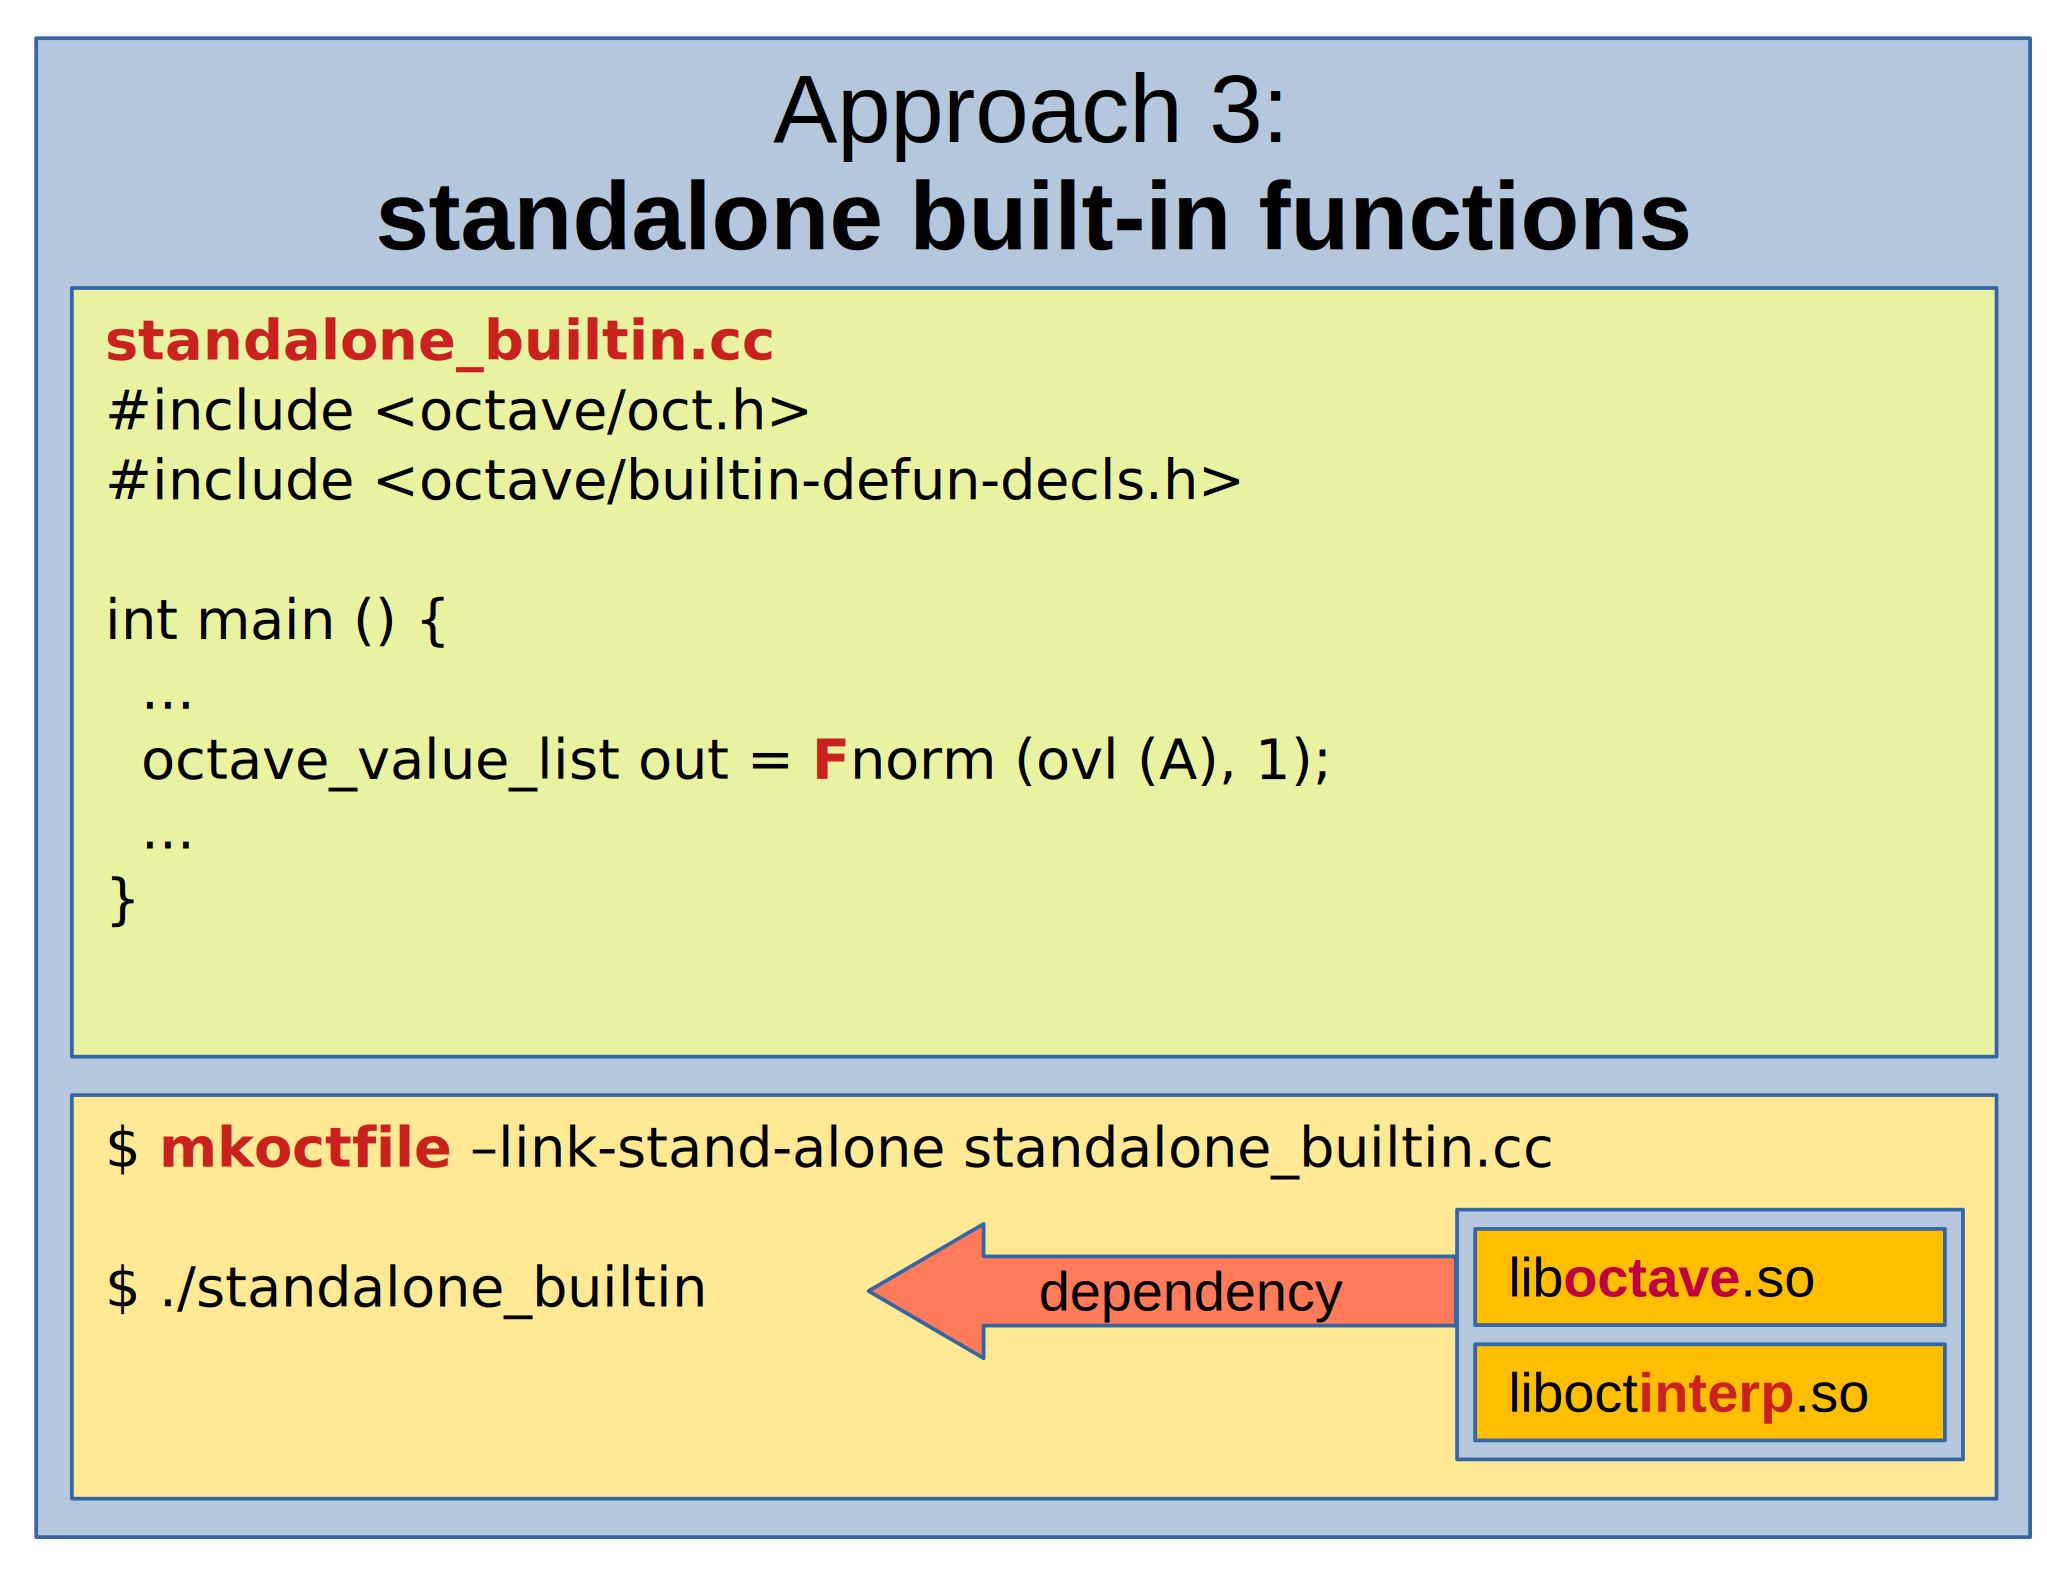
\includegraphics[width=\textwidth]{res/libreoffice/octave_c_cpp_fortran_3}
\end{column}
\begin{column}{0.4\textwidth}
\textbf{Problems to solve:}\\[0.8em]

\begin{itemize}
\itemsep1.5em
\item
My C/C++-program needs a functionality GNU Octave offers.
\begin{itemize}
\item
Using Octave's C/C++-code like any other C/C++-library.

\item
m-files are \textbf{NOT} supported.
\end{itemize}

\item
Code \textbf{interpretation} is for performance reasons not desired.
\end{itemize}
\end{column}
\end{columns}
\end{frame}



\begin{frame}{Advanced Octave usage - standalone applications (2/2)}
\begin{columns}
\begin{column}{0.5\textwidth}
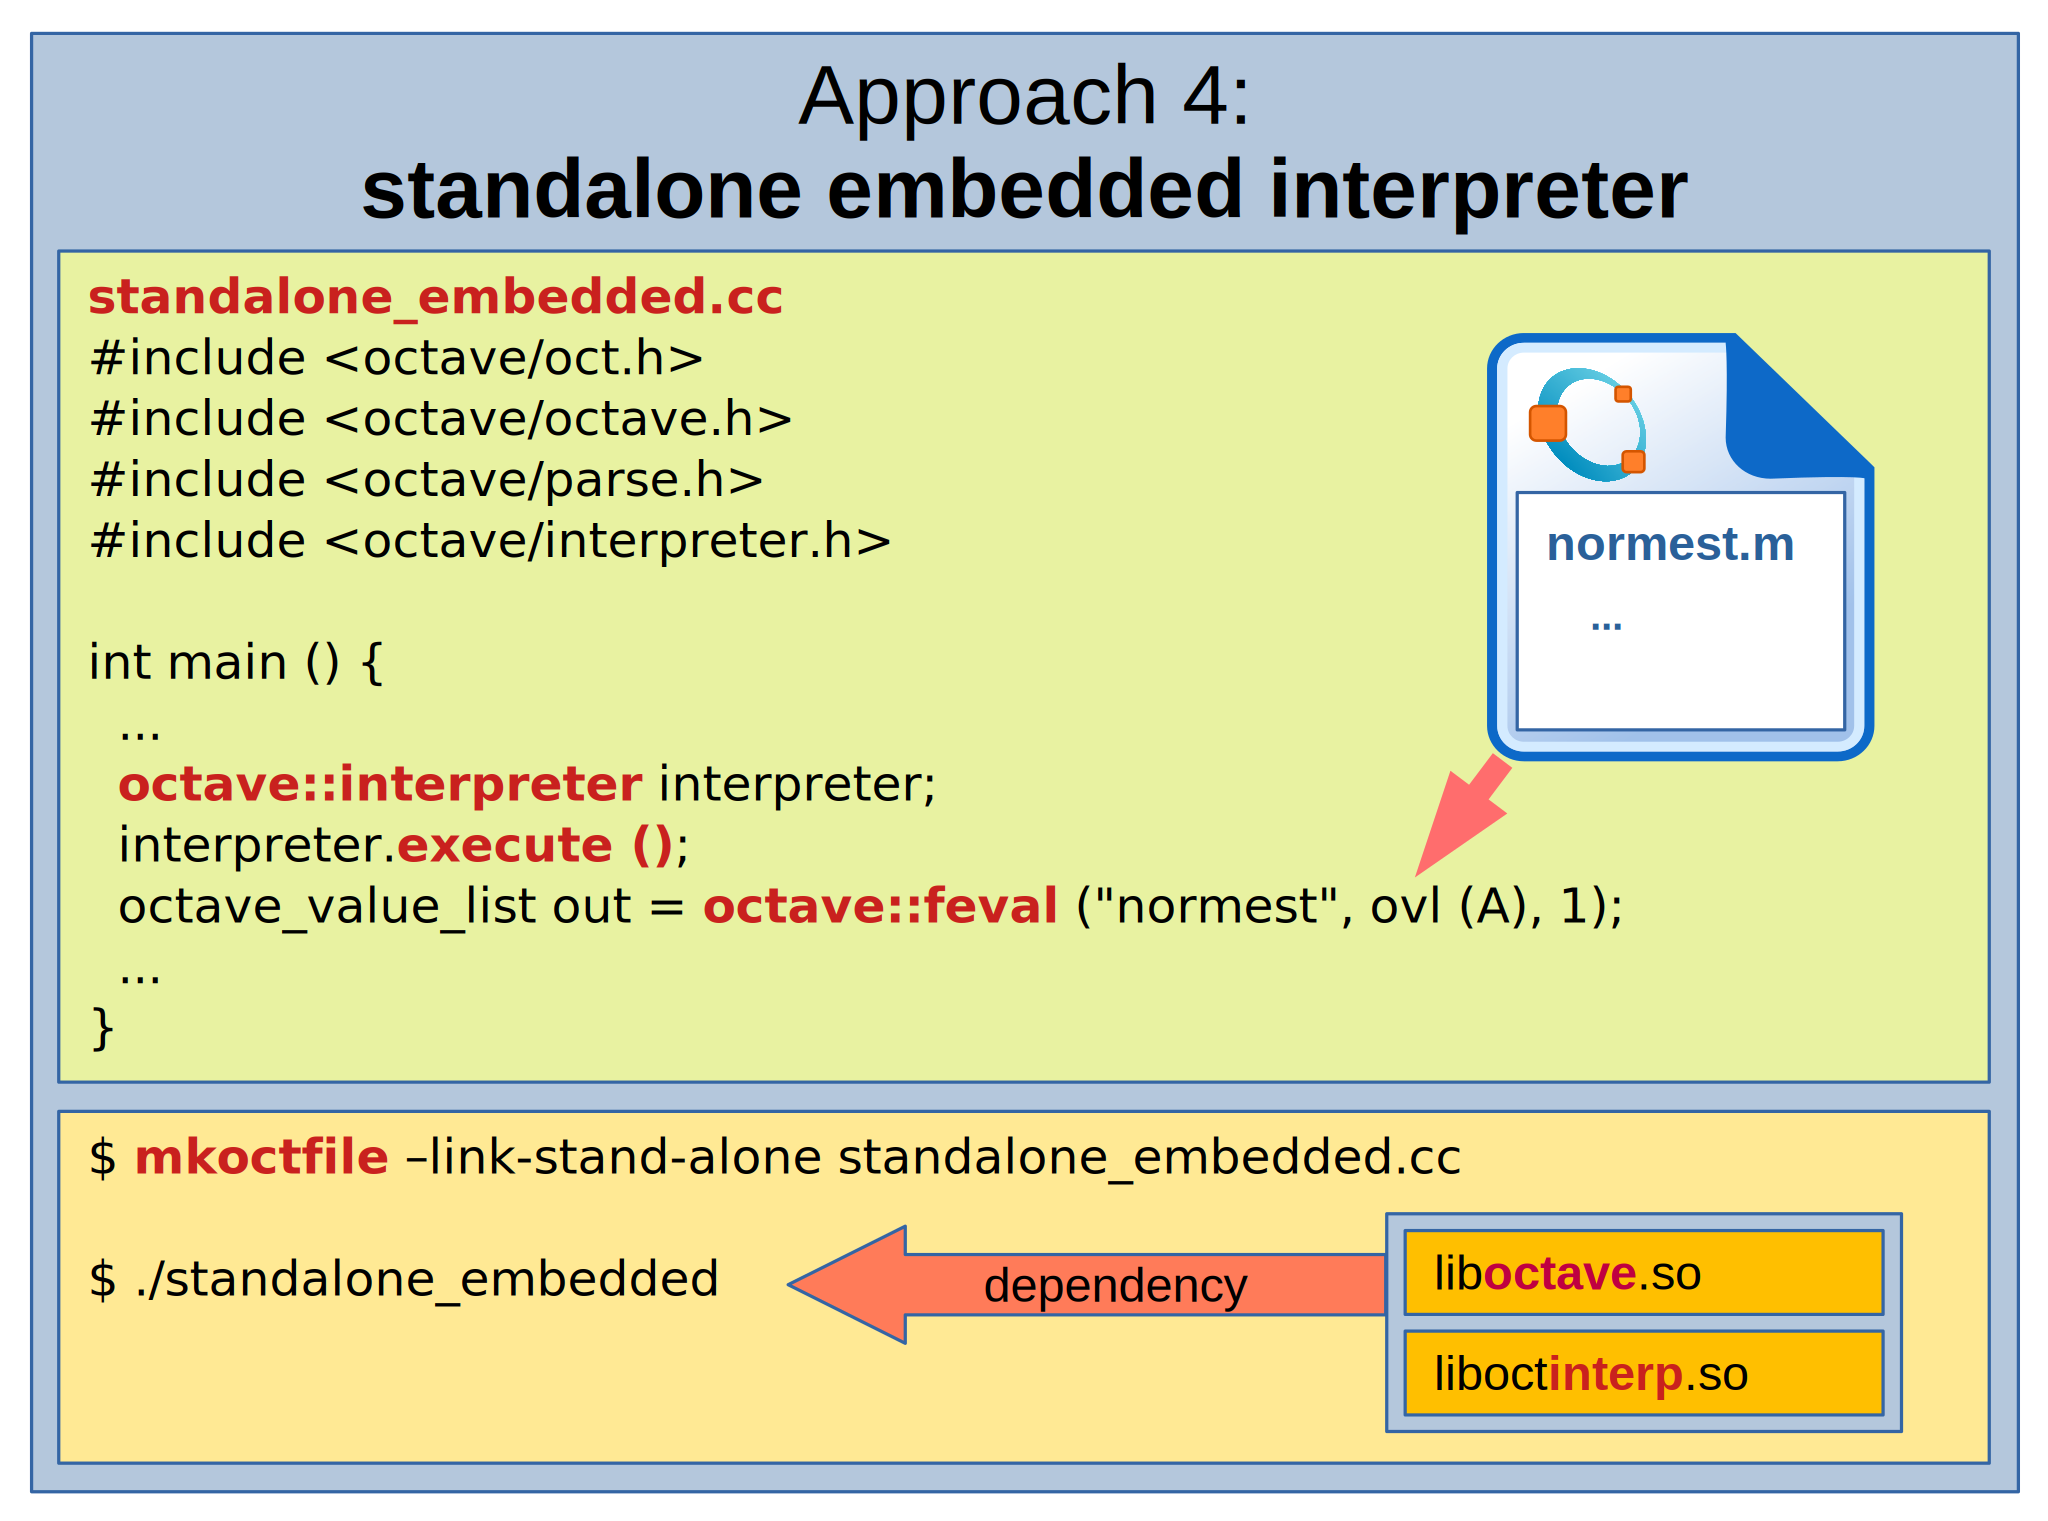
\includegraphics[width=\textwidth]{res/libreoffice/octave_c_cpp_fortran_4}
\end{column}
\begin{column}{0.4\textwidth}
\textbf{Problems to solve:}\\[0.8em]

\begin{itemize}
\itemsep1.5em
\item
My C/C++-program needs a functionality GNU Octave offers.
\begin{itemize}
\item
Using Octave's C/C++-code like any other C/C++-library.

\item
Using Octave's m-file functions via an interpreter.
\end{itemize}

\item
\textbf{Code/configuration flexibility}.
\begin{itemize}
\item
Change performance uncritical parts of the software without recompilation.
\end{itemize}
\end{itemize}
\end{column}
\end{columns}
\end{frame}


\begin{frame}{Advanced Octave usage (summary)}
\begin{columns}[t]
\begin{column}{0.15\textwidth}
\includegraphics[width=\textwidth]{res/libreoffice/octave_c_cpp_fortran_1}

\begin{itemize}
\item scripts
\item functions
\item classes
\item packages
\end{itemize}
\end{column}
\begin{column}{0.15\textwidth}
\includegraphics[width=\textwidth]{res/libreoffice/octave_c_cpp_fortran_2}
\begin{itemize}
\small
\item bring your own code
\item test your ideas
\end{itemize}
\end{column}
\begin{column}{0.3\textwidth}
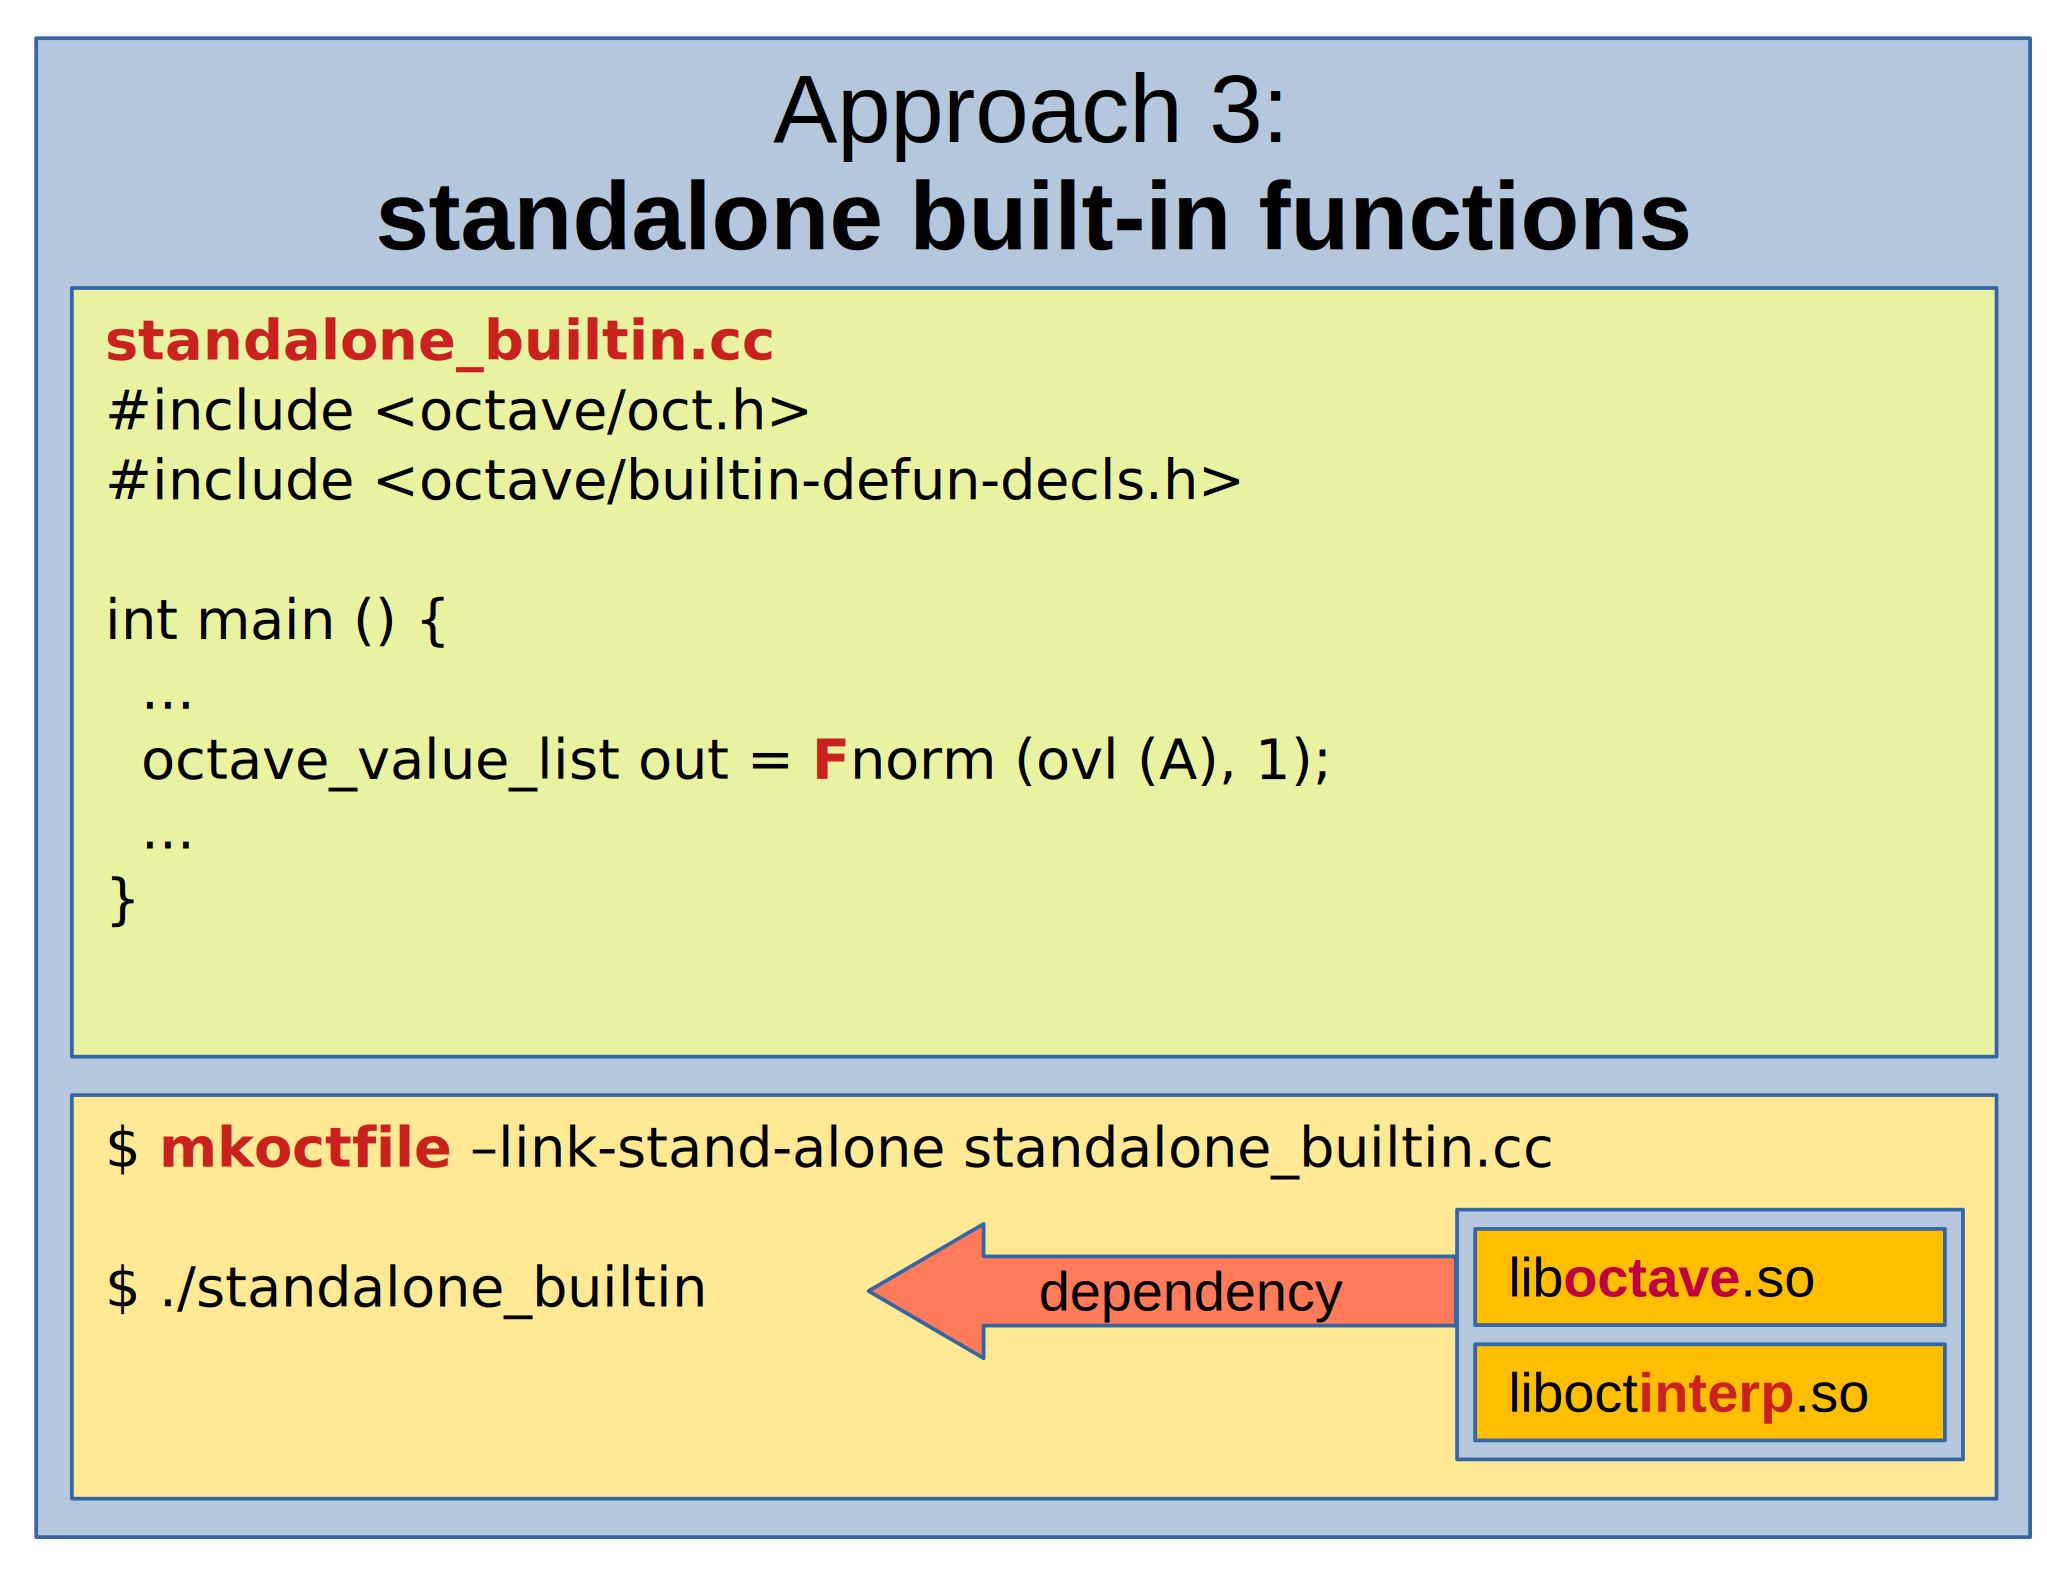
\includegraphics[width=\textwidth]{res/libreoffice/octave_c_cpp_fortran_3}
\begin{itemize}
\small
\item don't reinvent the wheel
\item \textbf{no m-files,\\ no interpreter!}
\end{itemize}
\end{column}
\begin{column}{0.3\textwidth}
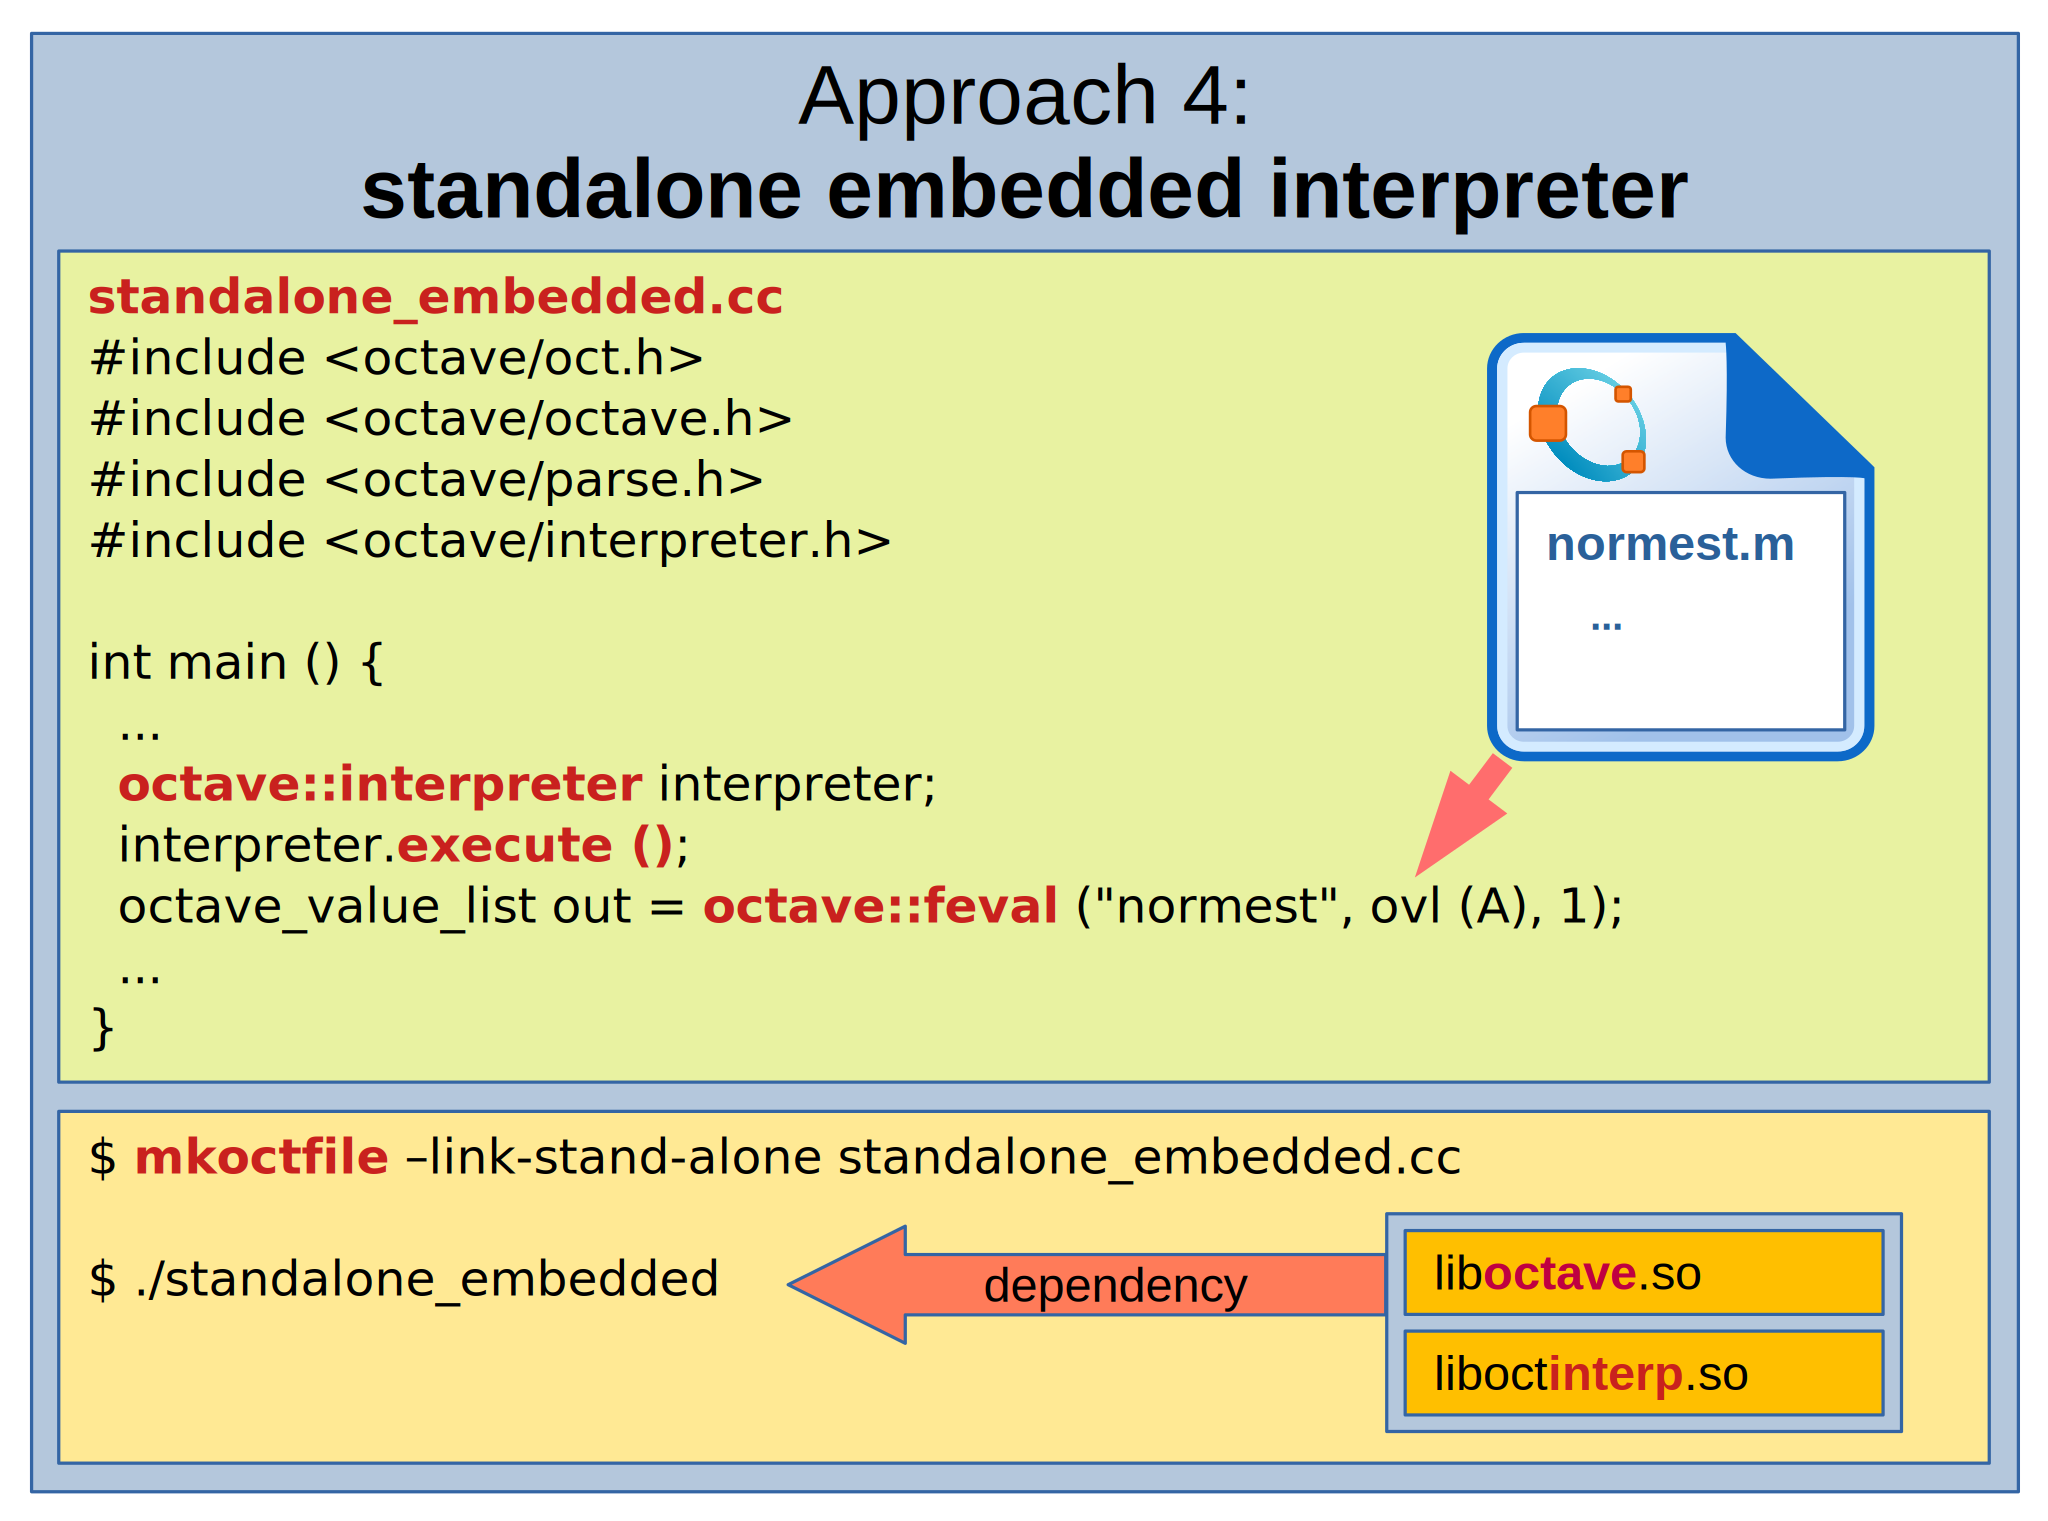
\includegraphics[width=\textwidth]{res/libreoffice/octave_c_cpp_fortran_4}
\begin{itemize}
\small
\item start your own Octave interpreter, when you need it
\end{itemize}
\end{column}
\end{columns}
\vfill
\colorbox{green!10}{\textbf{easy} \greencheck}
\hfill \colorbox{red!10}{\textbf{difficult}}
\end{frame}